% !TeX spellcheck = en_US
%\documentclass{beamer}
\documentclass[handout]{beamer}
\usepackage[spanish]{babel}
\usepackage[utf8]{inputenc}
\usepackage{graphicx}
\usepackage{multimedia}
\usepackage{animate}
\usepackage{tcolorbox}
\usebackgroundtemplate{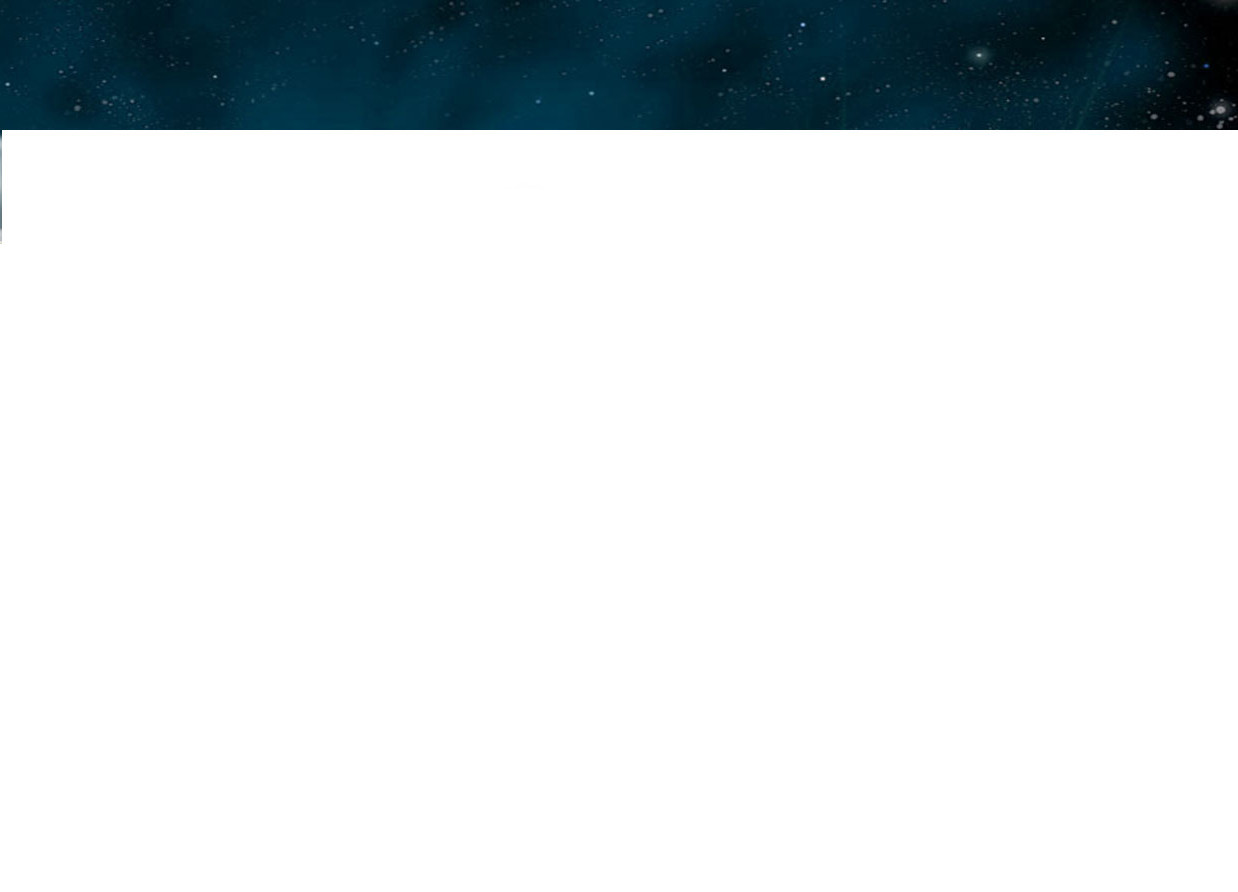
\includegraphics[width=\paperwidth]{sources/images/template_internal.jpg}}
\setbeamercolor{frametitle}{fg=white}
\usefonttheme{structuresmallcapsserif}
\setbeamertemplate{footline}[frame number]
\setbeamerfont{footnote}{size=\tiny}

\usepackage{default}

\usepackage[backend = bibtex, style = verbose, sorting = none, autocite = footnote]{biblatex}
\addbibresource{references.bib}

\newcommand\blfootnote[1]
{%
	\begingroup
	\renewcommand\thefootnote{}\footnote{#1}%
	\addtocounter{footnote}{-1}%
	\endgroup
}
\newcommand{\fcite}[1]{\blfootnote{\cite{#1}}}



\begin{document}
{
	\usebackgroundtemplate{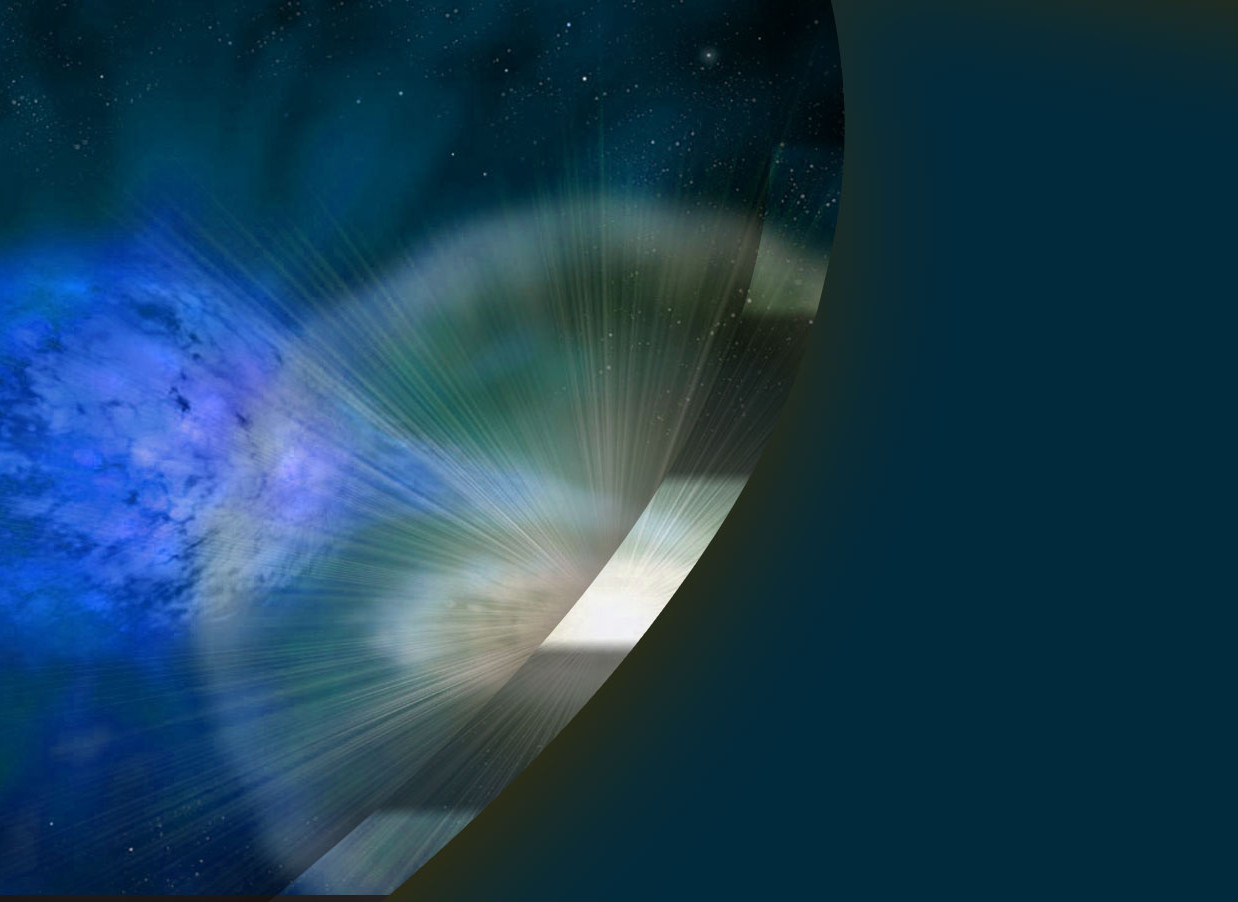
\includegraphics[width=\paperwidth]{sources/images/template_main.jpg}}
	\begin{frame}
		\centering
		\color{white}
		\textsc{\Huge El Universo Oscuro}
		\\
		\vspace{5cm}
		\raggedleft Juan Barbosa\\
		\raggedleft Seminario Avanzado
	\end{frame}
}

\begin{frame}{Introducci\'on}
	\centering
	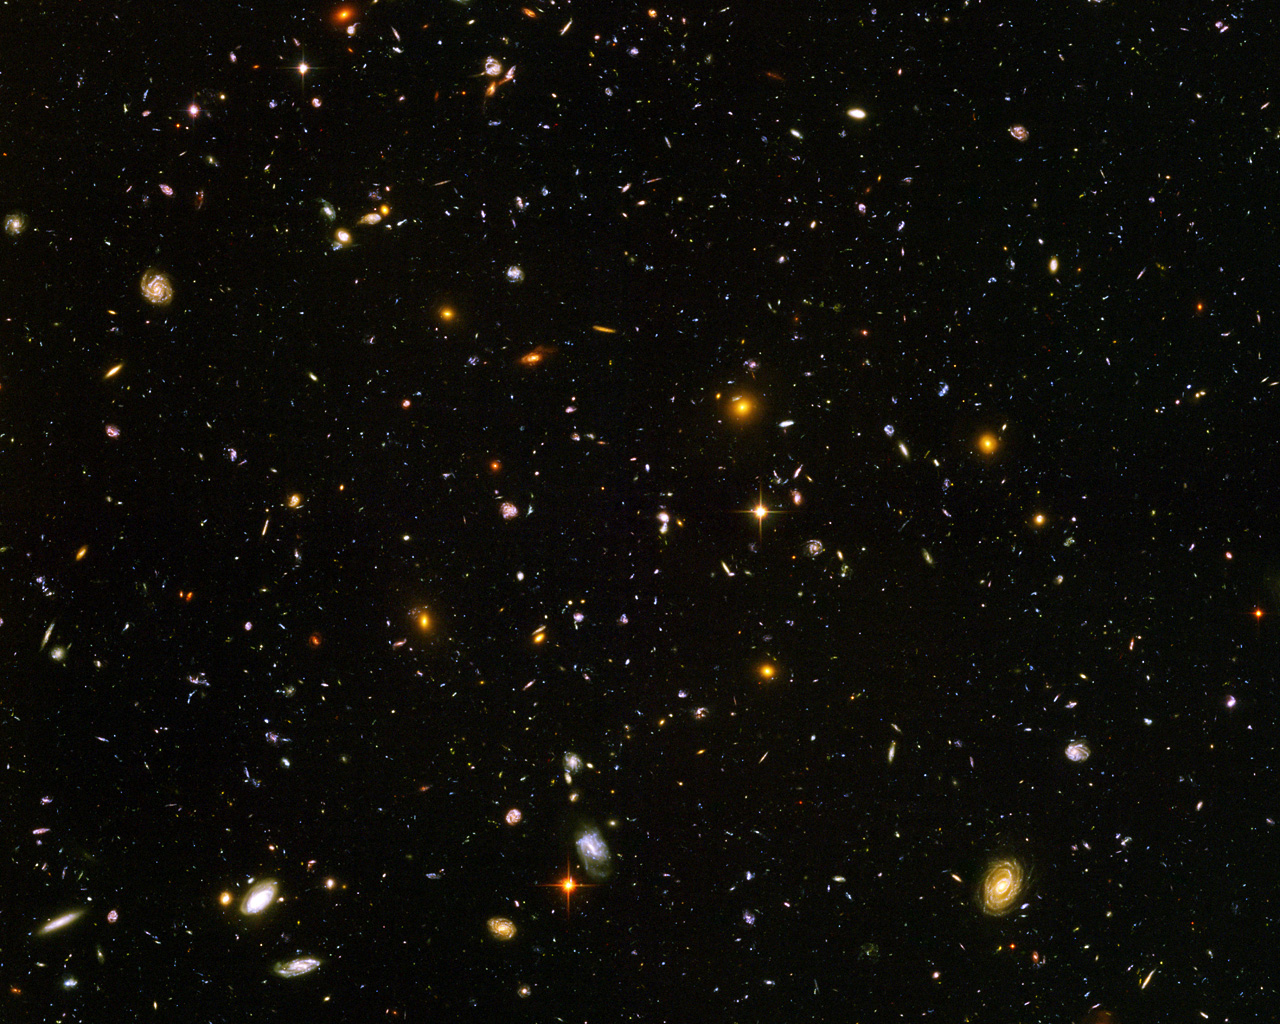
\includegraphics[height = 0.7\textheight]{sources/images/universe.jpg}
	\fcite{boker2002hubble}
\end{frame}

\begin{frame}{Estática y dinámica}
	\centering
	\begin{columns}
		\begin{column}{.5\textwidth}
			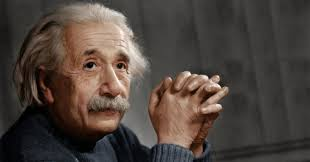
\includegraphics[width=\linewidth]{sources/images/einstein.jpg}
			
			En 1917 Albert Einstein publica su teoría de la relatividad general.
			\begin{equation}\footnotesize
				R_{\mu\nu} - \dfrac{1}{2}Rg_{\mu\nu} + \textcolor{red}{\Lambda} g_{\mu\nu} = \dfrac{8\pi G}{c^4}T_{\mu\nu}
			\end{equation}
			\begin{equation}\small
				\textcolor{red}{\Lambda} \neq 0
			\end{equation}
		\end{column}
		\begin{column}{.5\textwidth}
			\begin{figure}[h]
				\centering
				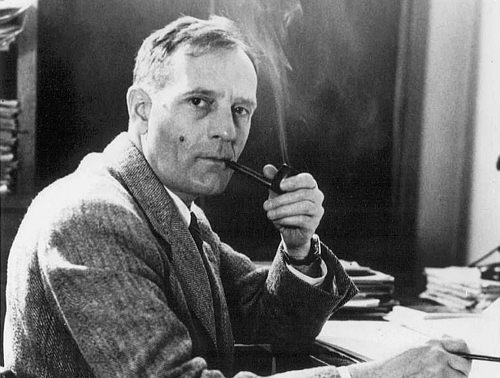
\includegraphics[width=0.6\linewidth]{sources/images/hubble.jpg}
			\end{figure}
			Para 1929 Edwin Hubble había demostrado que el universo estaba en expansión
			\begin{equation}
				cz = H_0d
			\end{equation}
		\end{column}
	\end{columns}
	\fcite{shirasaki2015probing}
\end{frame}

\begin{frame}{¿Cómo son posibles estas medidas?}
	Absorción atómica: para cada átomo un espectro
	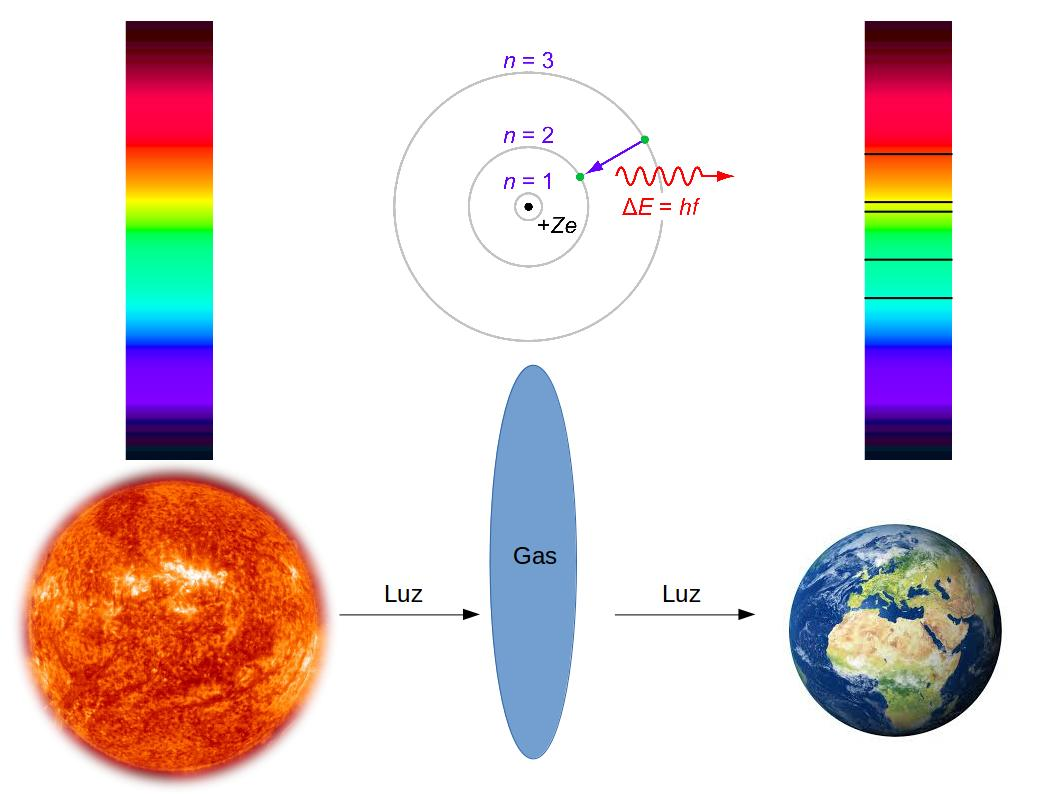
\includegraphics[height = 0.7\textheight]{sources/images/emission}
\end{frame}

\begin{frame}{¿Cómo son posibles estas medidas?}
	\begin{columns}
		\begin{column}{.3\textwidth}
			\vspace{5cm}
			\begin{equation}\small
				z = \dfrac{\lambda - \lambda_0}{\lambda_0}
			\end{equation}
		\end{column}
		\begin{column}{.6\textwidth}
			\begin{figure}[h]
				\centering
				\begin{tabular}{c}
					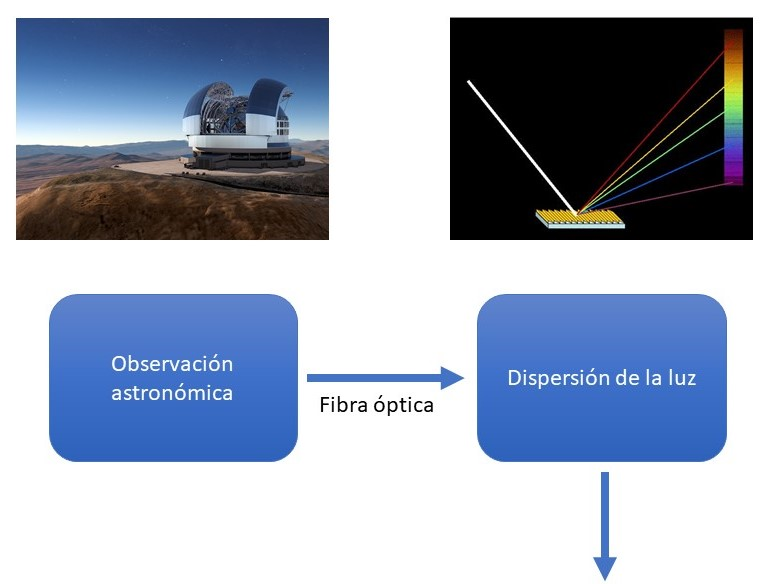
\includegraphics[height=0.5\textheight]{sources/images/measuring1.jpg} \\
					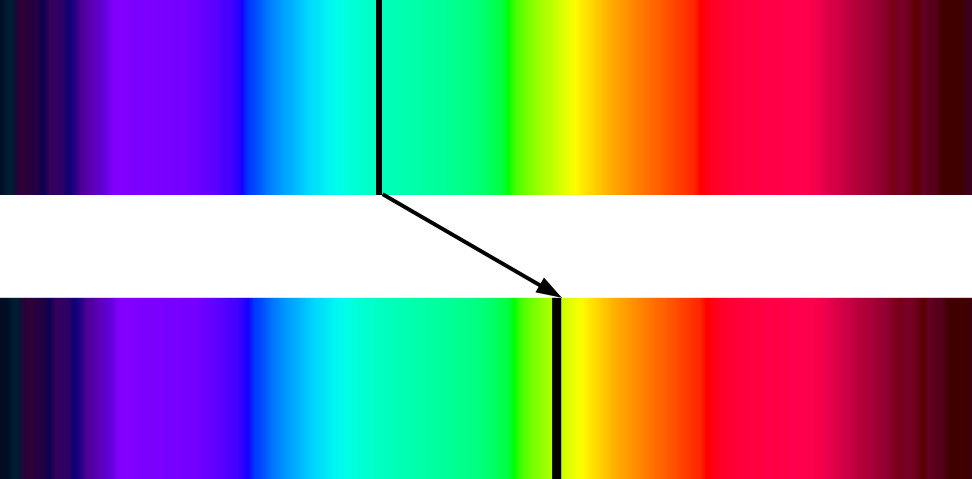
\includegraphics[width=0.6\linewidth]{sources/images/shift.jpg}
				\end{tabular}
			\end{figure}
		\end{column}
	\end{columns}
	\fcite{shirasaki2015probing}
\end{frame}

\begin{frame}{Resultados actuales}
	\centering
	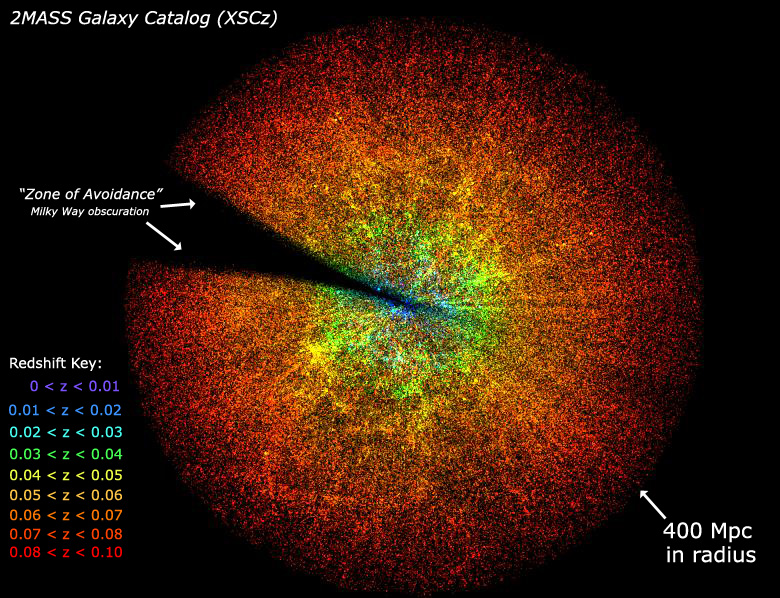
\includegraphics[width = 0.7\linewidth]{sources/images/2Mass.jpg}	
	\fcite{skrutskie2006two}
\end{frame}

\begin{frame}{Distribución del universo}
	\begin{columns}
		\begin{column}{0.5\textwidth}
			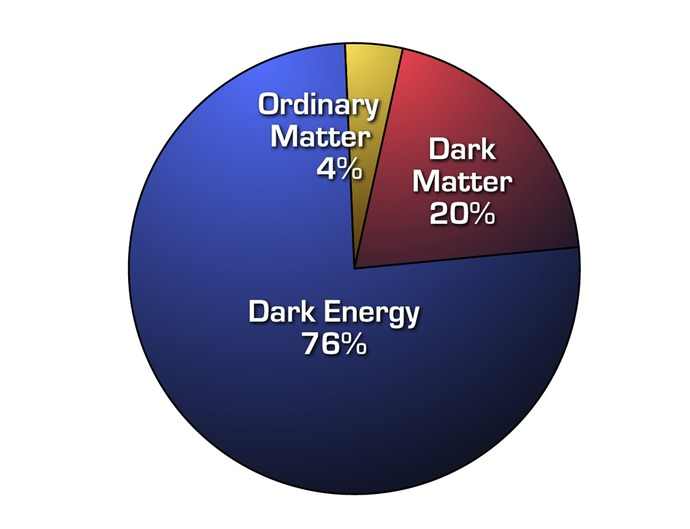
\includegraphics[width=\linewidth]{sources/images/udist.jpg}
		\end{column}
		\begin{column}{0.5\textwidth}
			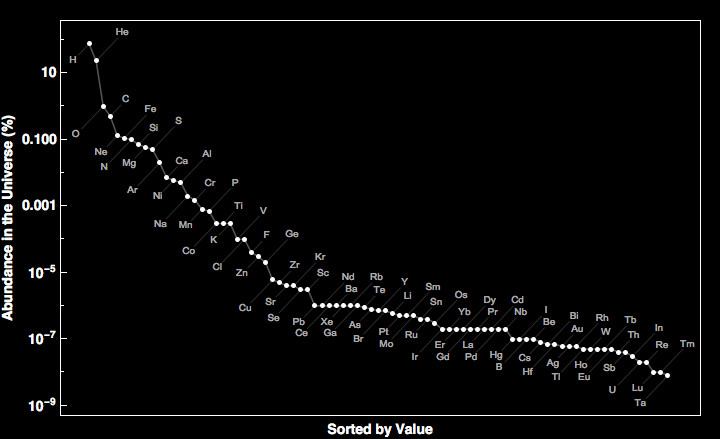
\includegraphics[width=\linewidth]{sources/images/edist.jpg}
		\end{column}
	\end{columns}
	\vspace{1cm}
	Nuestra comprensión de la naturaleza abarca el 4 \% del universo.
	\fcite{tegmark2006cosmological}
\end{frame}

\begin{frame}{Materia oscura}
	\begin{columns}
		\begin{column}{0.5\textwidth}
			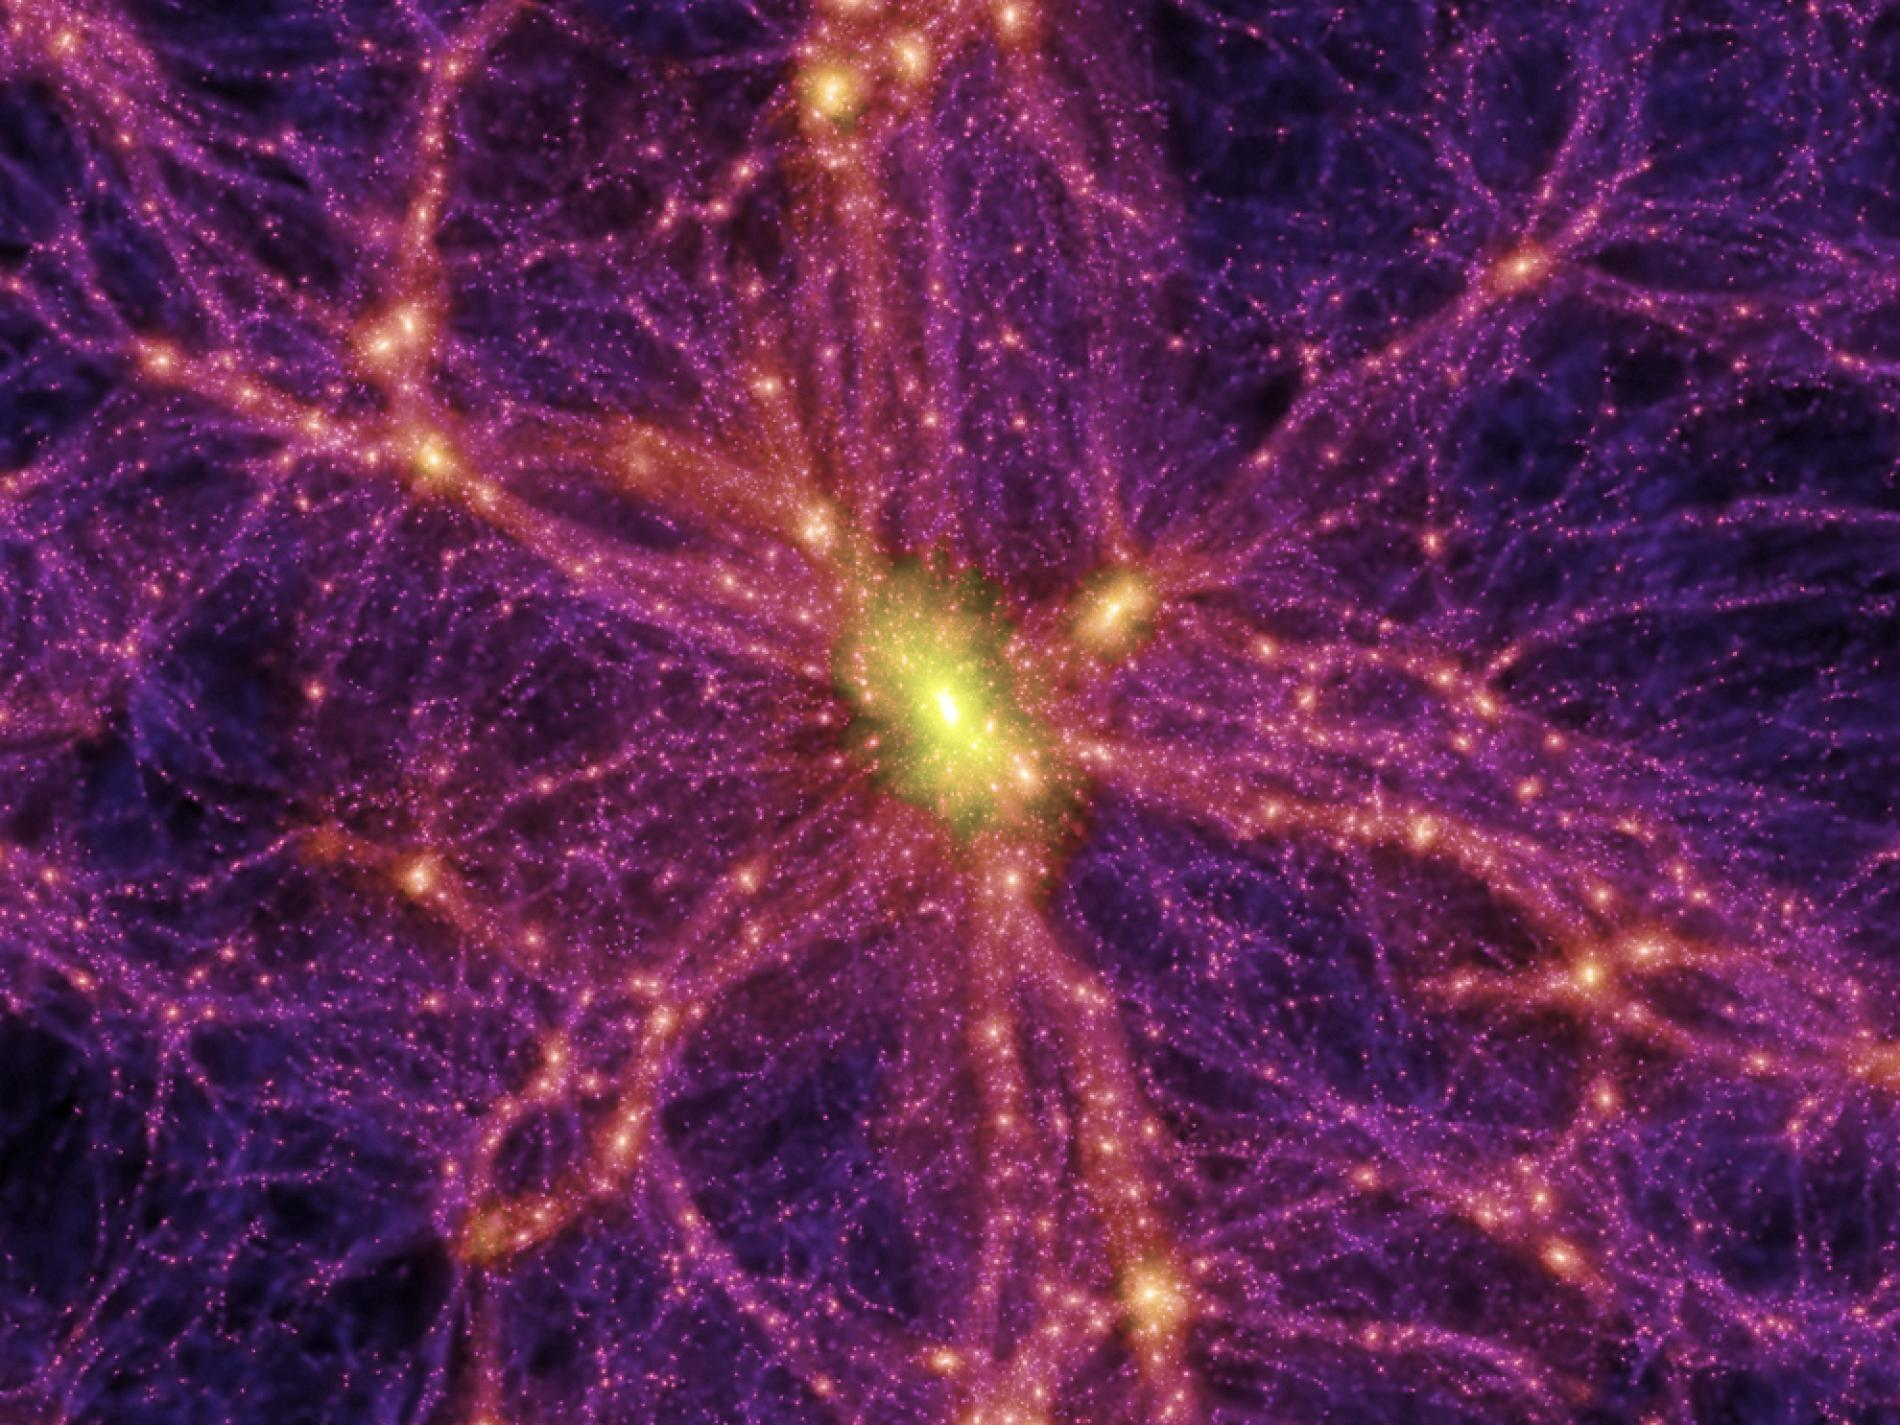
\includegraphics[width = \linewidth]{sources/images/natgeo.jpg}
		\end{column}
		\begin{column}{0.5\textwidth}
			Al igual que con la energía oscura, de la materia oscura sólo se conocen efectos indirectos.
			\begin{enumerate}
				\item Curvas de rotación de las galaxias
				\item Lentes gravitacionales
				\item Bullet cluster
			\end{enumerate}
		\end{column}
	\end{columns}
	\fcite{navarro1996structure}
\end{frame}

\begin{frame}{Rotación de las galaxias}
	\begin{columns}
		\begin{column}{0.6\textwidth}
			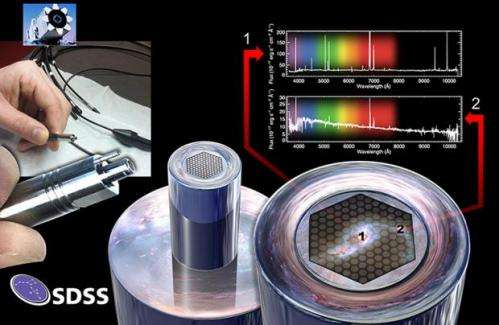
\includegraphics[width = 0.9\linewidth]{sources/images/SDSS.jpg} \\
			\begin{enumerate}
				\item Obtención del espectro en distintas regiones de la galaxia
				\item Caracterización del efecto Doppler
				\item Obtención de las velocidades
			\end{enumerate}
		\end{column}
		\begin{column}{0.4\textwidth}
			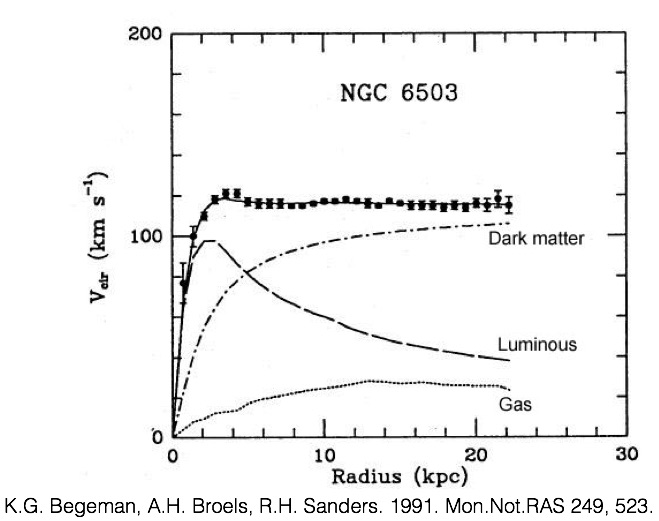
\includegraphics[width = \linewidth]{sources/images/rotation.jpg} \\
		\end{column}
	\end{columns}
	
	\fcite{tegmark2006cosmological}
\end{frame}

\begin{frame}{Lentes gravitacionales}
	\begin{columns}
		\begin{column}{0.6\textwidth}
			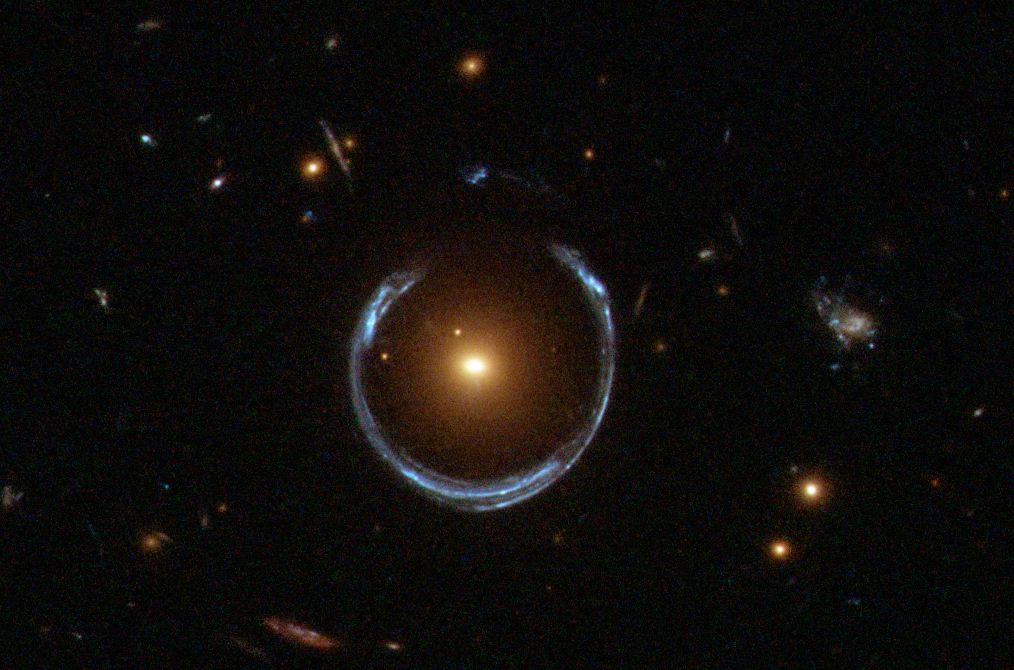
\includegraphics[width=\linewidth]{sources/images/Einstein_Ring.jpg}
			
			La luz no interactua con la fuerza gravitacional.
		\end{column}
		\begin{column}{0.4\textwidth}
			\begin{itemize}
				\item Objetos altamente masivos curvan el espacio-tiempo, modificando la trayectoria aparente de la luz.
				\item Sin embargo al contar la materia luminosa, su masa no es suficiente como para generar tal curvatura.
			\end{itemize}
		\end{column}
	\end{columns}
	
\end{frame}

\begin{frame}{Lentes gravitacionales}
	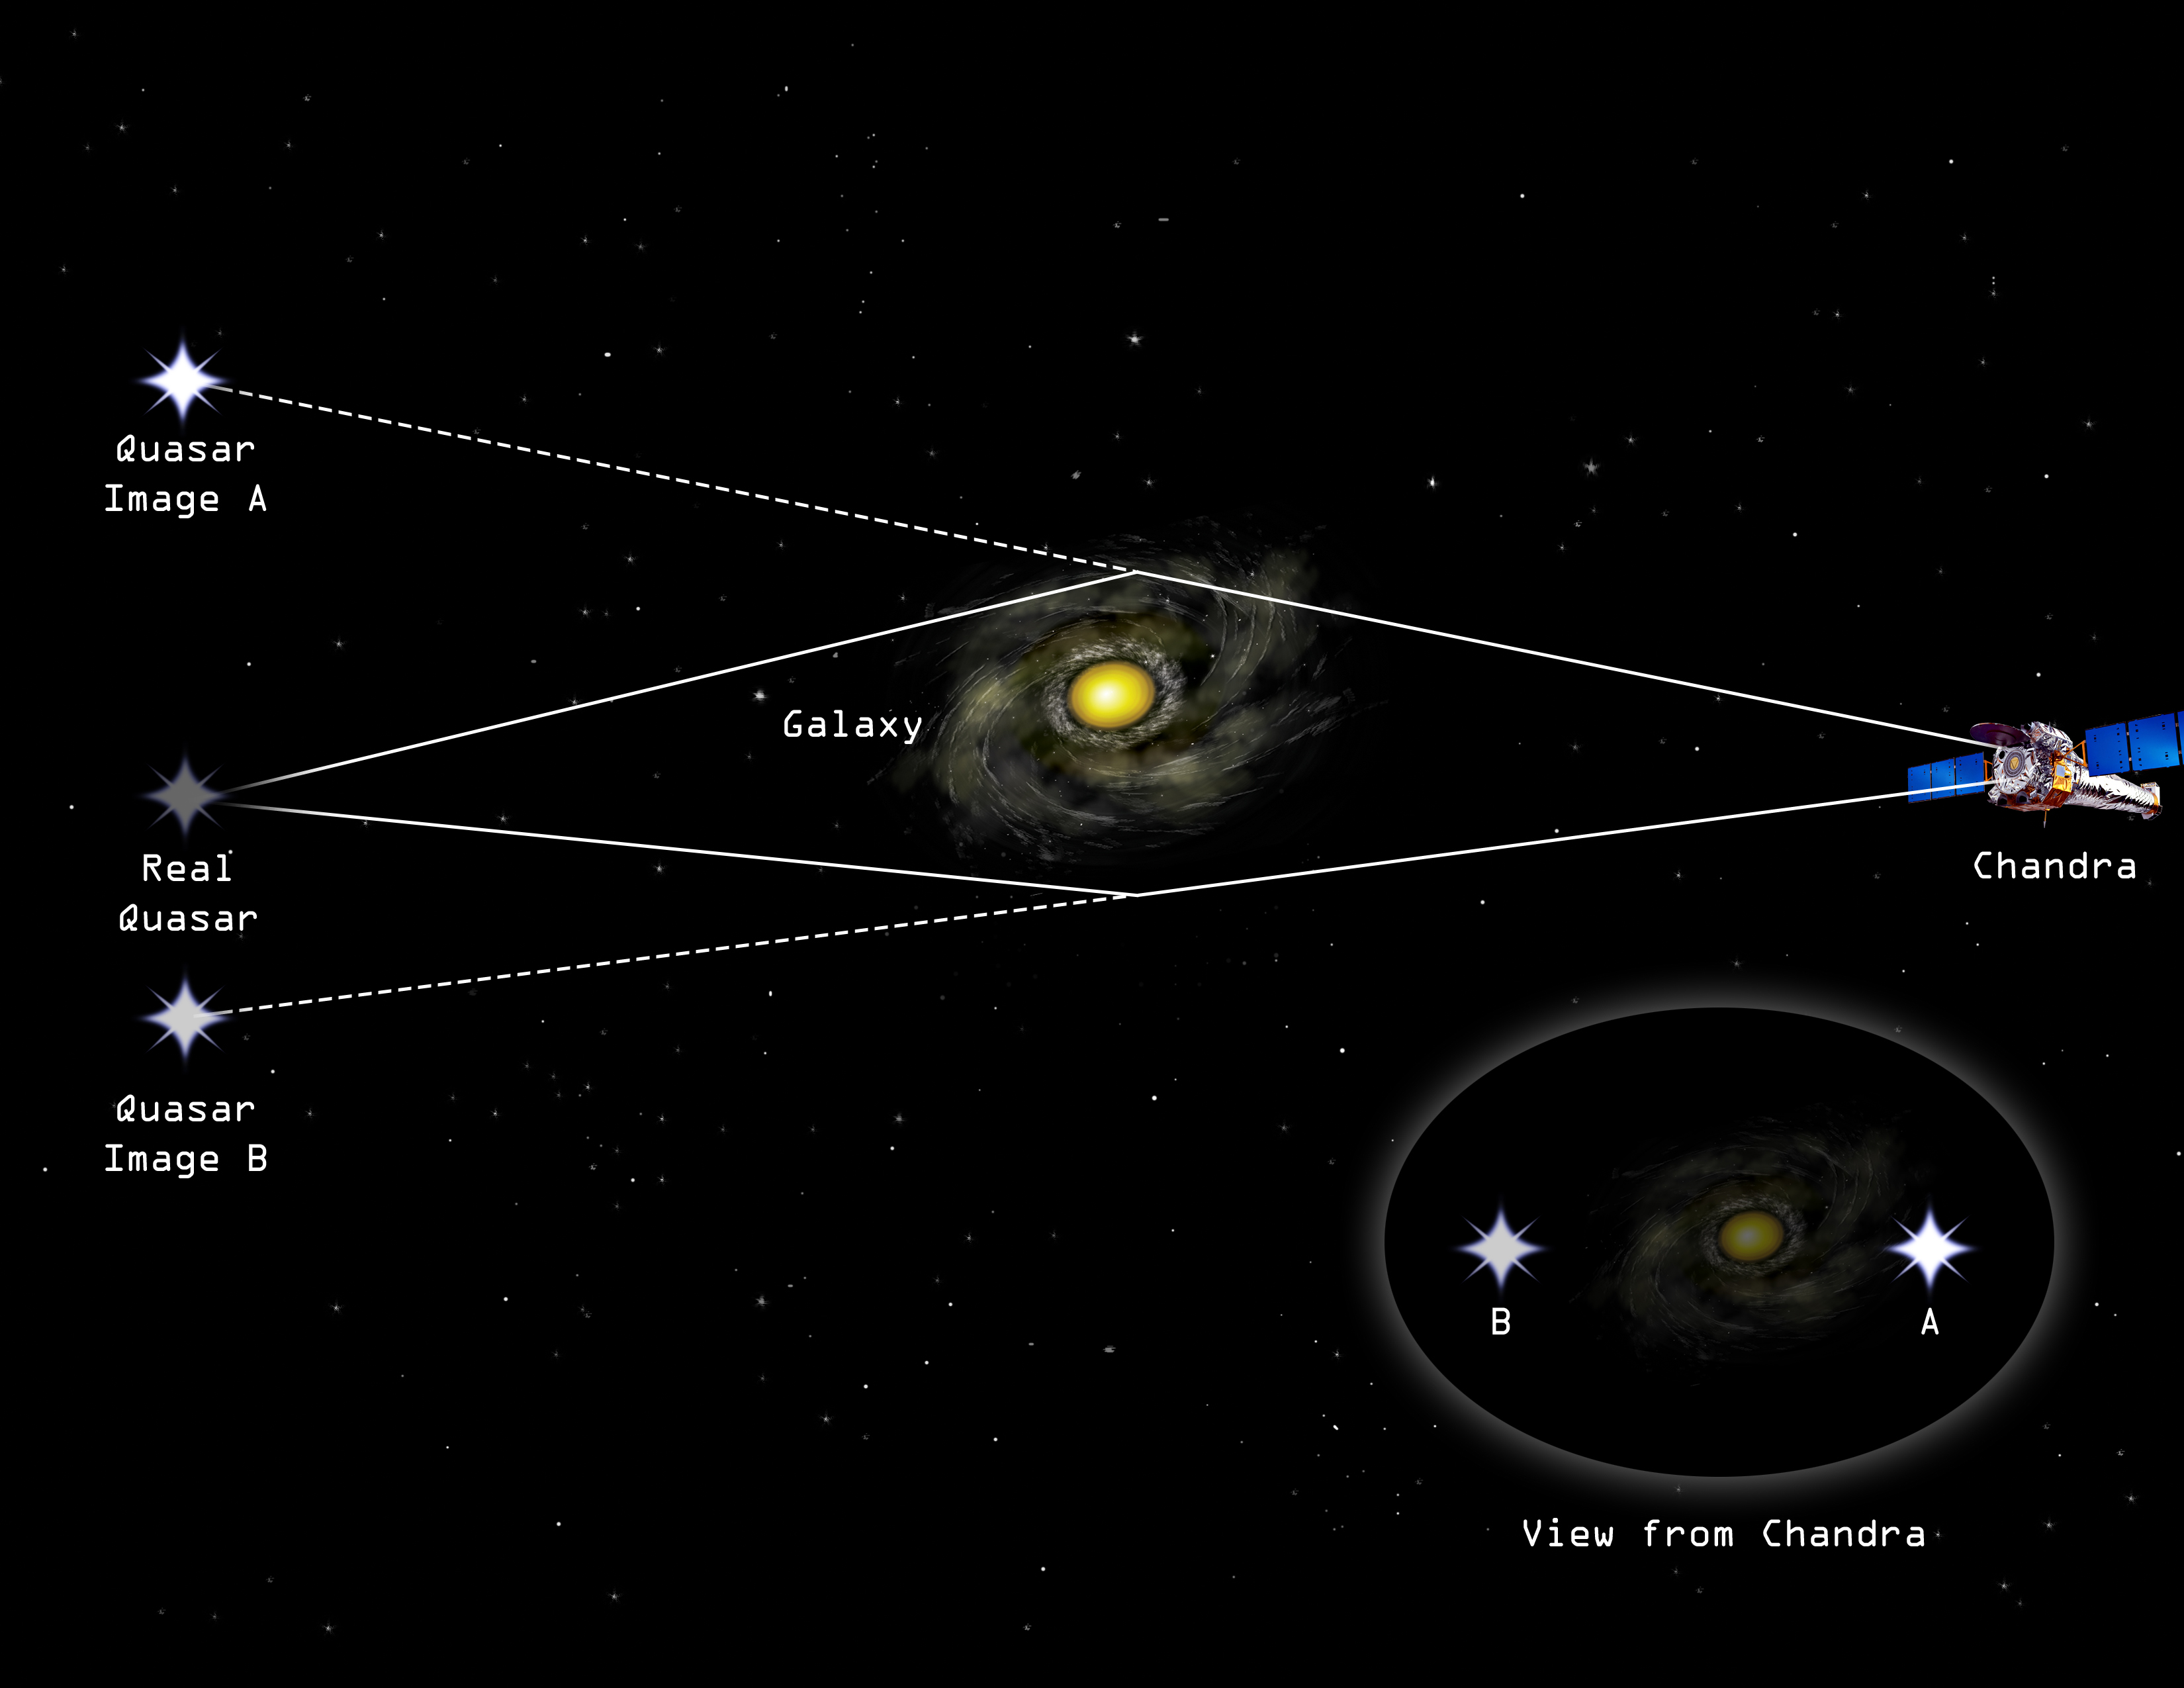
\includegraphics[width = 0.7\linewidth]{sources/images/lens.jpg}
	
\end{frame}

\begin{frame}{Bullet cluster}
	Colisión de dos clusters de galaxias
	\begin{columns}
		\begin{column}{0.4\textwidth}
			\begin{itemize}\small
				\item \textbf{Rosado:} rayos X
				\item \textbf{Azul:} distribución de masa
			\end{itemize}
		\end{column}
		\begin{column}{0.6\textwidth}
			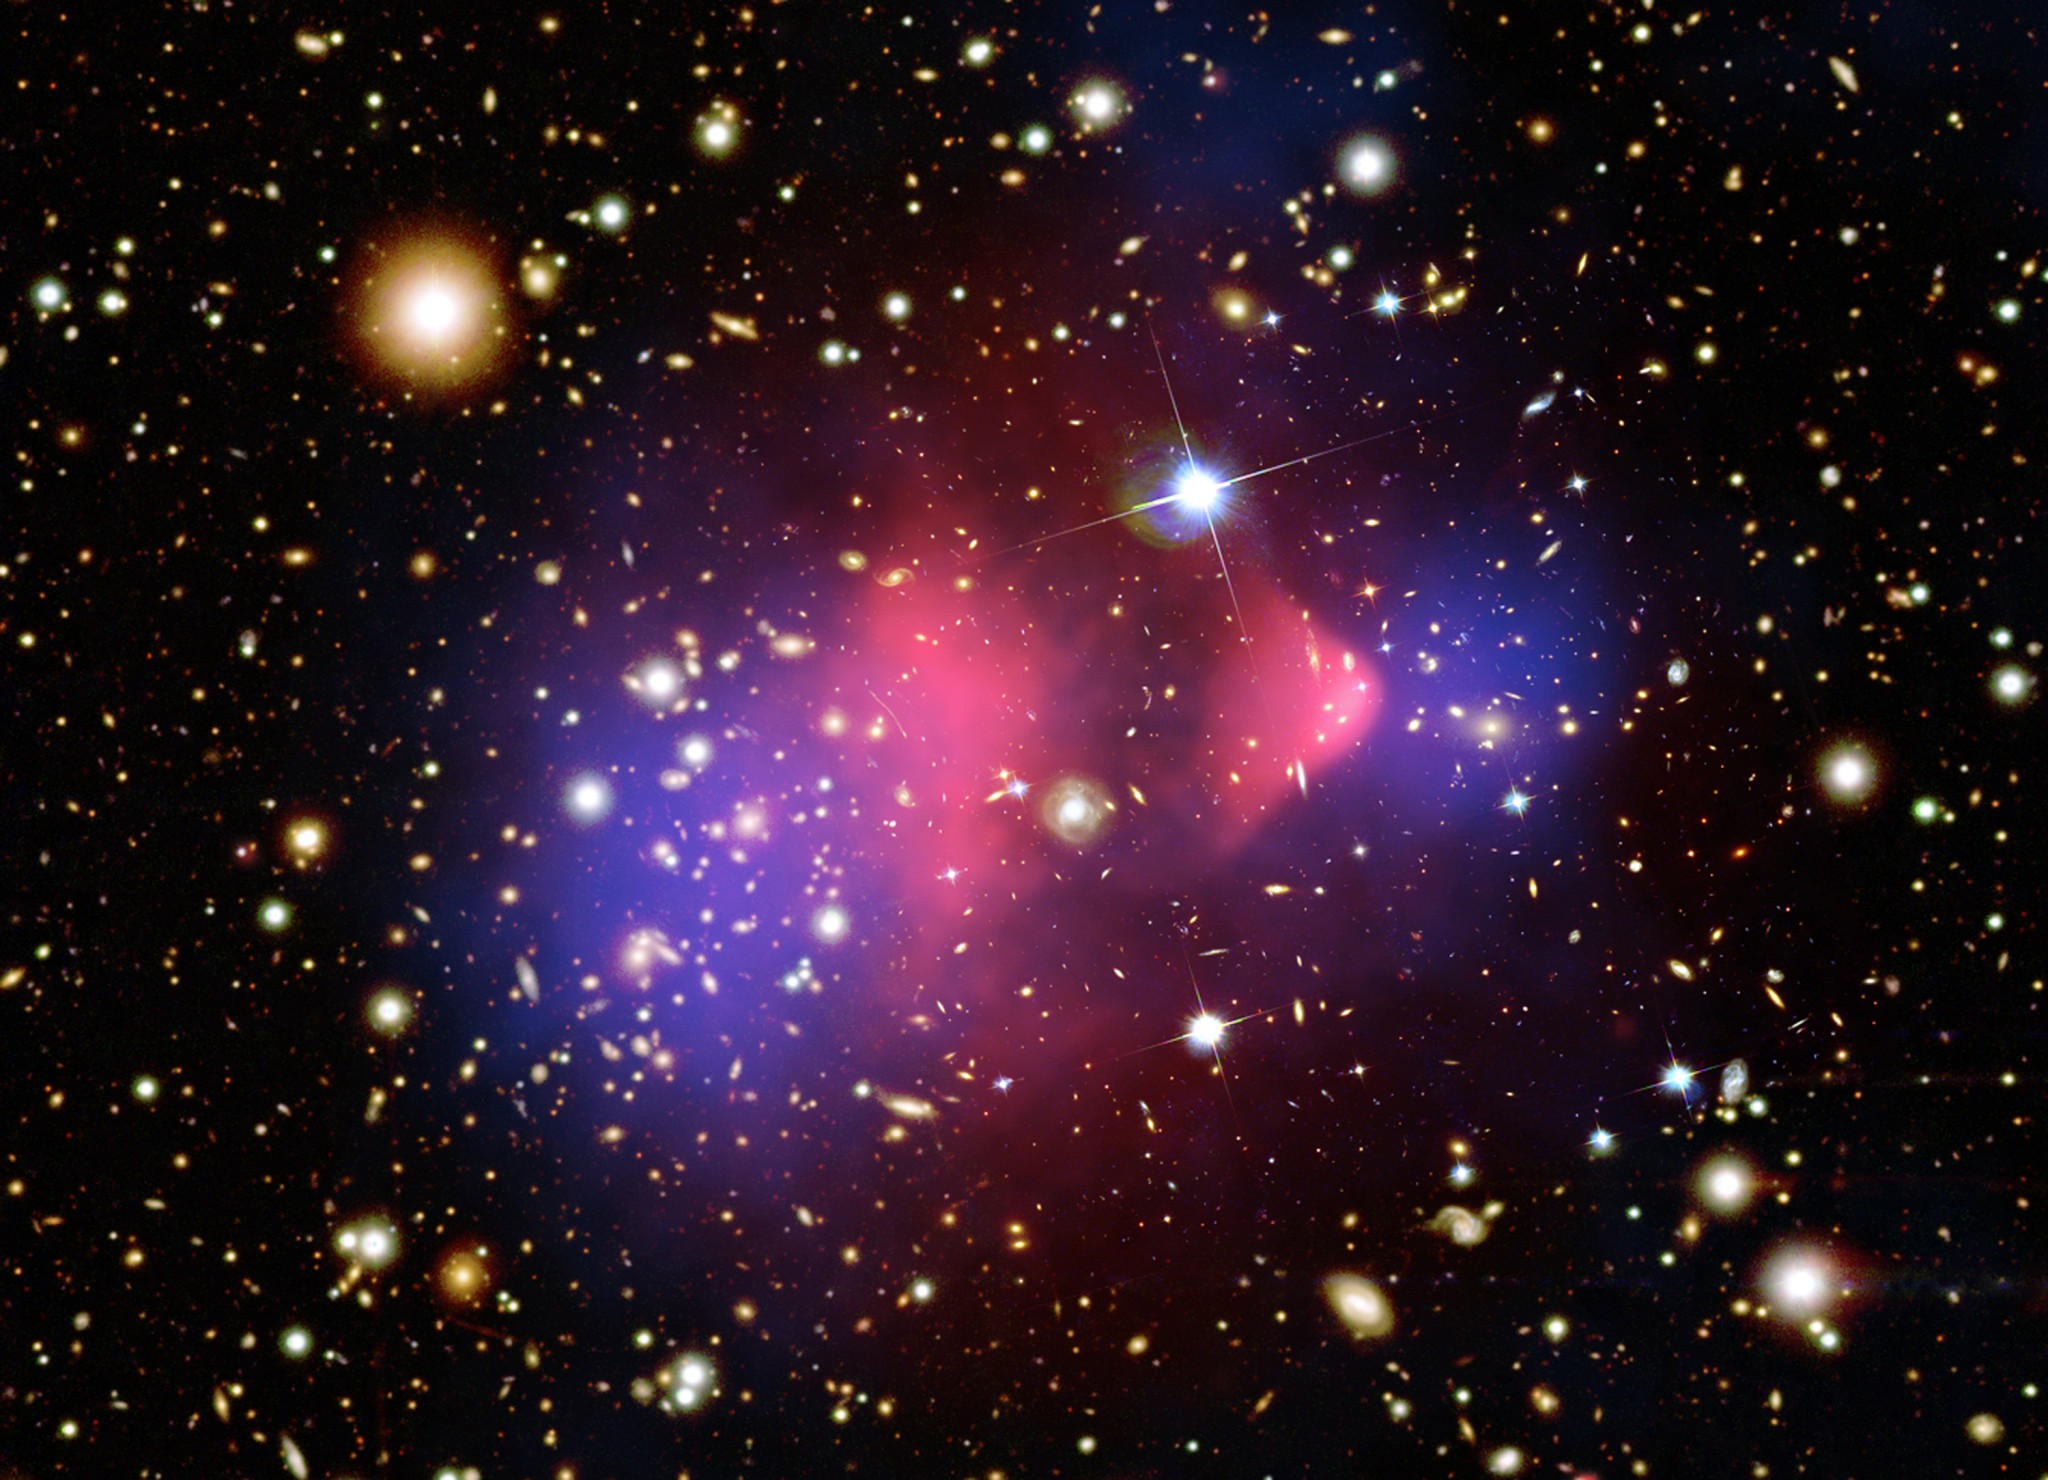
\includegraphics[width = \linewidth]{sources/images/bullet}
		\end{column}
	\end{columns}
	\fcite{brownstein2007bullet}
\end{frame}

\begin{frame}{Bullet cluster}
	\vspace{1cm}
	{\footnotesize
		\url{https://www.youtube.com/watch?v=rLx_TXhTXbs}
	}
\end{frame}

\begin{frame}{¿Qué es la materia oscura?}\small
	\begin{figure}[h]
		\centering
		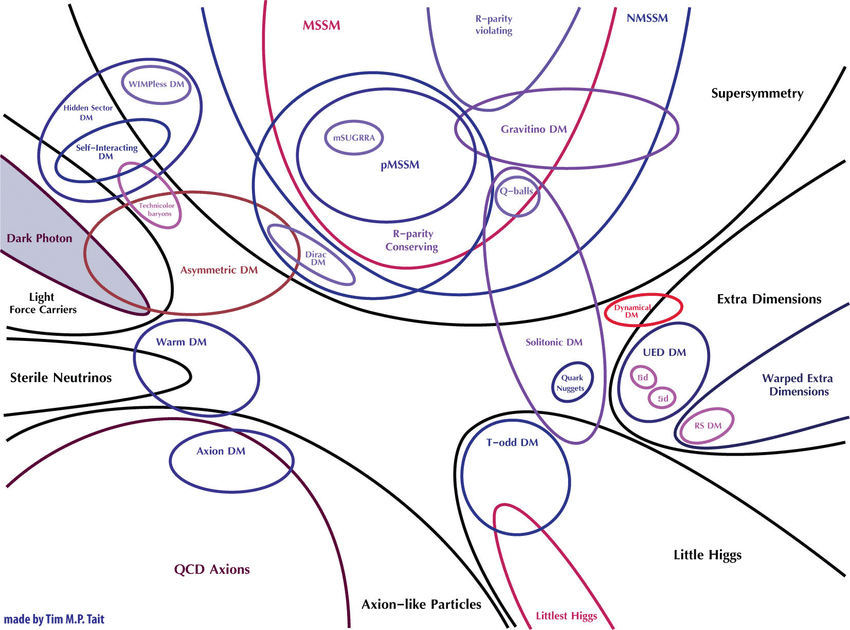
\includegraphics[width = 0.7\linewidth]{sources/images/candidates}
	\end{figure}
	
	Una enorme cantidad de partículas han sido propuestas como candidatas a la materia oscura, sin embargo, ningún experimento ha detectado una de ellas. 
\end{frame}
\end{document}